\chapter{Программая реализация разработанного метода нечеткого вывода с применением технологии CUDA}\label{ch:ch3}

Для удобства реализация выполнялась не постредством прямого использованием API библиотеки CUDA, а с помощью шаблонной библиотеки реализации высокопроизводительных вычислений - \textbf{Kokkos} \ref{}, предназначенной для портативного и эффективного параллельного программирования на различных аппаратных архитектурах, включая многоядерные процессоры, графические процессоры NVIDIA/AMD и другие ускорители. Интерфейс библиотеки позволяет абстрагироваться от деталей низкоуровневого параллелизма, позволяя разработчикам писать код на C++ с одним исходным кодом, который может быть оптимизирован для различных платформ без существенных изменений. 
Ключевые функциональные возможности библиотеки упростившие выполнение программного реализации разработанного ранее метода:
\begin{itemize}
\item Модели параллельного выполнения: абстрагирование параллельных циклов (например, "parallel\_for", "parallel\_reduce") и рабочих процессов на основе задач.  
\item Управление памятью: Автоматизированная обработка пространств памяти (например, между хостом и устройством) и расположением данных для оптимизации схем доступа и минимизации объема передаваемых данных.  
\item Поддержка серверной части: интеграция с такими моделями программирования, как CUDA, HIP, OpenMP и SYCL, для обеспечения кроссплатформенной совместимости.  
\item Переносимость производительности: Обеспечивает эффективное использование ресурсов (потоки, векторизация) с учетом особенностей каждой архитектуры.
\end{itemize}

Kokkos широко используется в научных вычислениях и HPC-приложениях, упрощая разработку масштабируемых кодов при сохранении производительности на постоянно развивающемся оборудовании. 

При выполнении процедуры нечеткого вывода для набора входных данных можно выполнять процедуру вывода по каждому входному экземпляру независимо, то есть параллельно. Кроме того можно предусмотреть отбор небольшого в сравнении с общим количеством ограниченного подмножества правил нечеткой системы, наиболее релевантных входному экземпляру. Сам алгоритм нечеткого вывода не предусматривает наличия промежуточной информации, котой бы нужно было обмениваться между вычислениями по другим экземплярам входных данных. Тогда, поскольку алгоритм нечеткого вывода для каждого экземпляра входных данных можно реализовать при ограниченном небольшом объеме входных и промежуточных данных, имеет смысл разместить эти данные в памяти предоставляющей наибольшую скорость обращения, которая в технологии CUDA соответствует динамической памяти внутри CUDA-блока, а сами вычисления над этими данными также реализовать внутри этого CUDA-блока.



\section{Вычисление нечеткого значения истинности с помощью дискретизации функций принадлежностей}\label{sec:ch3/sect1}

\begin{figure}[hbt]
	\centering
   	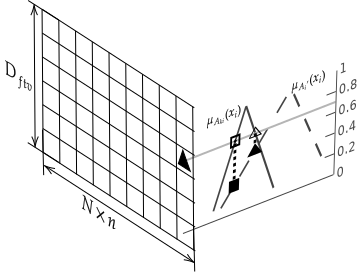
\includegraphics[width=0.6\textwidth]{ftv-opengl-computation.pdf}
	\label{ftv-opengl-computation}
\end{figure}

\begin{figure}[hbt]
	\centering
   	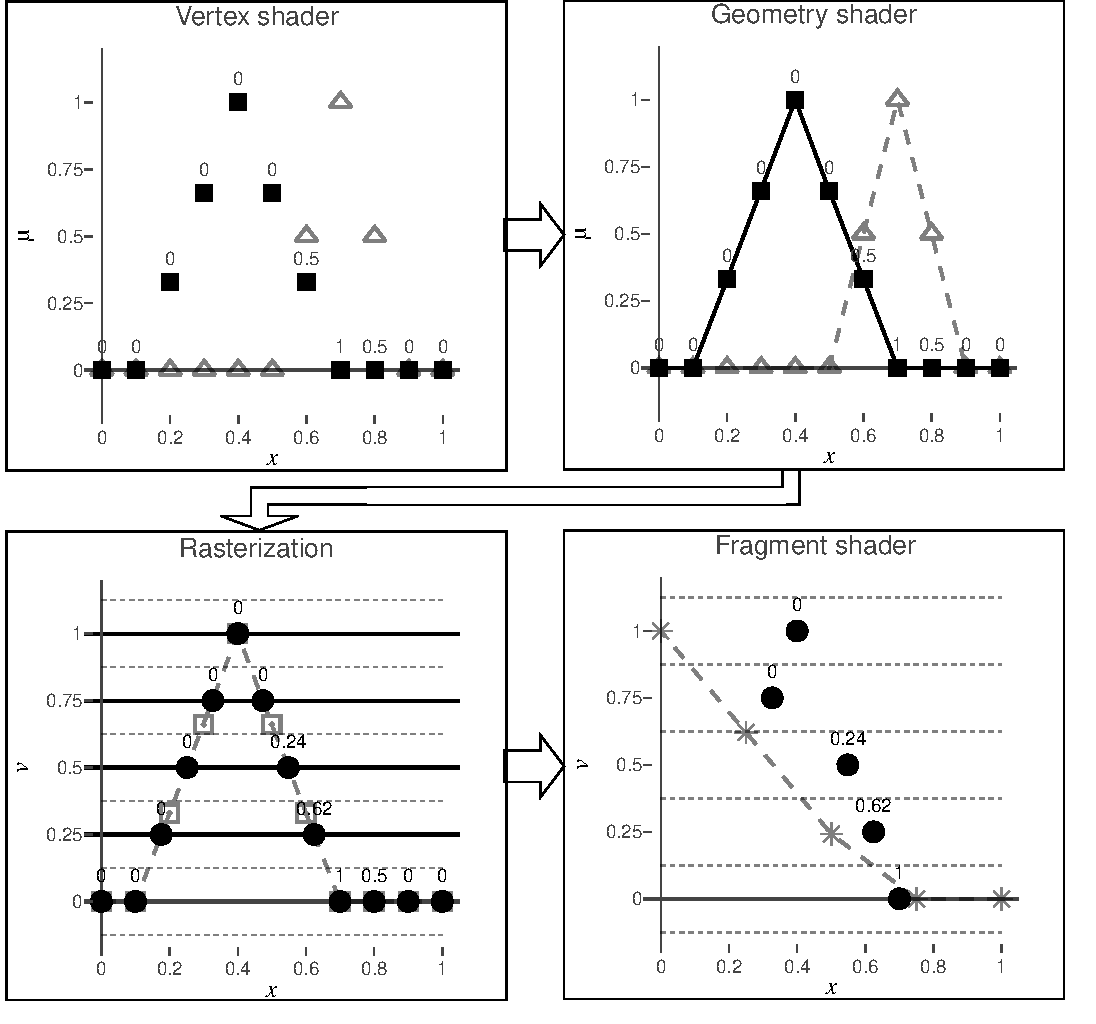
\includegraphics[width=1.0\textwidth]{ftv-opengl-computation-pipeline.pdf}
	\label{ftv-opengl-computation-pipeline}
\end{figure}

\section{Алгоритм свертки НЗИ при $T_1=min$ и $T_3$ - неубывающая по всем аргументам}\label{sec:ch3/sect2}

\begin{algorithm}
\label{alg:ftv-reduction}
\begin{algorithmic}
\Require $ftv_i,\ i=\overline{1,n}$
\State $max\_ftv[i] = 0;$
\For{$v = 1\dots0$}
\State $s \gets \left\{ftv_i[v] \mid ftv_i[v] >= max\_ftv[i]\right\};$
\State $max\_ftv[i] \gets max(max\_ftv[i], ftv_i[v]);$
\State $v\_max \gets \max_{i}\left\{ftv_i[v]\right\}, v\_max\_index \gets \mathrm{arg\,max}_i\left\{ftv_i[v]\right\};$
\If{$s = \emptyset \And i = v\_max\_index$}
\State $r[i] \gets v\_max;$
\Else
\State $r[i] \gets max\_ftv[i];$
\EndIf
\State $ftv[v] \gets \underset{i}{T_3}\left\{r[i]\right\}$;
\EndFor
\State \Return $ftv$
\end{algorithmic}
\caption{Алгоритм свертки НЗИ при $T_1=min$ и $T_3(a, b) \ge T_3(c, d)$ если $a > c$ или $b > d$}
\end{algorithm}

\begin{figure}
    \label{fig:ftvs-reduction-example}
    \centering
    \includegraphics[width=15cm]{ftvs-reduction-example.pdf}
    \caption{Иллюстрация работы алгоритма свертки НЗИ для нескольких входов для расширенной $\mathrm{\tilde{T}}$-нормы при $T_1=\mathrm{min}$ и $T_3=\mathrm{min}$.}
\end{figure}

При 

\pgfplotsset{
    axis grid/.style={
        width=0.3\textwidth,
        height=0.3\textwidth,
        domain=0:1,
    }
}

\begin{figure}
	\centering
	\begin{tikzpicture}[
	    % Style for column headers (above each column)
	    column header/.style={
	        anchor=south,
	        font=\bfseries,
	        yshift=10pt
	    },
	    % Style for row headers (left of each row)
	    row header/.style={
	        anchor=east,
	        font=\bfseries,
	        xshift=-10pt,
	        rotate=90
	    }
	]
		\matrix[row sep=0.5cm, column sep=0.1cm] (mat) {
			\node[] {}; &
			\node[column header] {$\tau_{A_k|A'} =$ <<АБСОЛЮТНО ЛОЖНО>>}; &
			\node[column header] {Column 1}; &
			\node[column header] {Column 1}; \\
			
			\node[row header] {$\mu_{B_k}(y) = 0$}; &
			\begin{axis}[axis grid]
				\addplot {(1-x)^2};
			\end{axis} &
			\begin{axis}[axis grid]
			\end{axis} &
			\begin{axis}[axis grid]
			\end{axis} \\
		};
	\end{tikzpicture}
\end{figure}

\section{Реализация дефаззификации}

Нахождение начального приблежения

\section{Использование библиотеки ArborX}\label{sec:ch3/sect2}

\begin{figure}[hbt]
	\label{fig:z-curve-apetrei}
	\centering
	\begin{minipage}[b]{0.45\textwidth}
		\centering
		\includegraphics[width=\textwidth]{z-curve}
		\caption*{(a) z-curve}
	\end{minipage}\hfill
	\begin{minipage}[b]{0.45\textwidth}
		\centering
		\includegraphics[width=\textwidth]{apetrei}
		\caption*{(b) apetrei}
	\end{minipage}
	\caption{Две иллюстрации: графика z-curve и apetrei.}
\end{figure}

В \cite{prokopenko2024revisingapetreisboundingvolume} авторами библиотеки \textbf{ArborX} предложен алгоритм для эффективного построения \textit{иерархии ограничивающих объемов}. Данная структура данных используется для эффективного поиска ближайшей точки в $n$-мерном пространстве. Алгоритм выполняет построение структуры поиска за $O(N\times log(N))$, где $N$ - количество точек в исходном наборе. Логика поиска места в иерархии ограничивающих объемов для каждой отдельной точки помещена в отдельную нить параллельных вычислений, после чего остается ятолько логирифмическая компонента сложности, соответствующая восходящему обходу промежуточного дерева и помещения точки в подобранный узел \fixme{с использованием атомарной операции}. В основе алгоритма лежит группировка близко расположенных точек для более быстрого подбора соответствующего ограничивающего объема за счет проецирования точки из $n$-мерного пространства на $Z$-кривую посредством вычисления кода Мортона для каждой точки. Согласно эвристике, лежащие рядом на $Z$-кривой точки располагаются достаточно близко и исходном $n$-мерном пространстве. Кроме того в статье описан модифицированный алгоритм Апетрея [], обеспечивающий обход иерархии на этапе поиска ближайших точек без необходимости помещения цепочки пройденных родительских узлов в стек за счет передачи информации об альтернативных узлах-кандидатах из родительских узлов в дочерние. Такой подход значительно снижает количество потребляемой памяти для сохранения промежуточной информации при выполении этапа поиска.

\section{Алгоритм построения базы правил}

